\documentclass[12pt]{article}

%%% Shared preamble (packages, fonts, layout)
\usepackage{linguistics-preamble}
\addbibresource{../../Bibliography/references.bib}

%%% Paper-specific commands
\newcommand{\sltag}[1]{\ensuremath{\boxed{#1}}}

%%% Title
\title{The Acceptability of Symbiotic Gaps}
\author{Michael Dover and Masaya Yoshida}
\date{March 11, 2026}

\begin{document}
\maketitle

%% ==========================================================
%% SECTION 1: INTRODUCTION
%% ==========================================================

\section{Introduction}

Parasitic gap constructions \citep{ross1967,engdahl1983,culicover2001} have served as a productive empirical domain for evaluating theories of filler-gap dependencies. In the canonical case, illustrated in (\ref{intro-pg}), a single filler is associated with two gaps: one in a position from which extraction is independently possible (the ``true'' gap) and another inside an island (the ``parasitic'' gap).

\ex\label{intro-pg} Which articles did you file \underline{\hspace{1em}} [without reading \underline{\hspace{1em}}]?
\xe

\noindent The label ``parasitic'' reflects the dependent nature of the island-internal gap: it can be licensed only in the presence of the true gap. On movement-based analyses, this dependency follows from the requirement that a primary extraction chain be established from a non-island position before the parasitic gap can be licensed \citep[see, e.g.,][]{chomsky1982,chomsky1986,kayne1983,nunes2004}.

\citet{levine2003} challenge this picture by presenting a class of sentences they call \emph{symbiotic gap} constructions. In these examples, gaps occur inside both a subject island and an adjunct island, with no gap in the matrix verb's complement position. \citeauthor{levine2003} argue that the apparent mutual dependency between the two gap sites cannot be captured by any analysis that requires an asymmetric licensing relationship between gaps. They contend that HPSG \citep{pollard1994}, which treats all gaps in a sentence through a single uniform mechanism, handles symbiotic gaps just as naturally as standard parasitic gaps, and should therefore be preferred to movement-based alternatives.

In this paper, we present experimental evidence from an acceptability judgment task that undermines the empirical foundation of this argument. Our results show that symbiotic gap sentences receive low acceptability ratings, at levels comparable to or worse than sentences involving clear island violations. Crucially, when a third gap is introduced in the matrix verb's complement position, acceptability improves significantly. This improvement indicates that the matrix gap plays an essential licensing role: without it, the island-internal gaps cannot be licensed.

These findings recast the theoretical debate. If symbiotic gaps are not well-formed, then the inability of movement-based theories to generate them is a correct prediction rather than a shortcoming. Conversely, the capacity of HPSG to generate symbiotic gap configurations becomes a case of overgeneration rather than an empirical advantage. Since a grammar should exclude symbiotic gap sentences, movement-based approaches are to be preferred. The paper proceeds as follows. Section~\ref{sec:background} reviews the relevant data and theoretical background, examining three movement-based approaches (the null operator/connectedness analysis, the predicate modification approach, and sideward movement) alongside the HPSG account. Sections~\ref{sec:experiment} and~\ref{sec:experiment2} present two acceptability judgment experiments. Section~\ref{sec:discussion} discusses the theoretical implications. Section~\ref{sec:conclusion} concludes.

%% ==========================================================
%% SECTION 2: BACKGROUND
%% ==========================================================

\section{Background}\label{sec:background}

\subsection{Parasitic gaps}\label{sec:bg-pg}

Parasitic gap constructions are unbounded dependency constructions in which a single filler is associated with two gaps. The parasitic gap may appear inside an adjunct island, as in (\ref{bg-pg-a}), or inside a subject island, as in (\ref{bg-pg-b}).

\pex
\a\label{bg-pg-a} Which articles$_i$ did you file \underline{\hspace{1em}}$_i$ [without reading \underline{\hspace{1em}}$_i$]?
\a\label{bg-pg-b} Which candidate$_i$ did [supporters of \underline{\hspace{1em}}$_i$] end up voting for \underline{\hspace{1em}}$_i$?
\xe

\noindent In both cases, the true gap occupies the matrix verb's complement position, a site from which extraction is independently well-formed. The island-internal gap is parasitic on this true gap: filling the matrix complement position while leaving only the island-internal gap results in unacceptability, as (\ref{bg-no-true}) shows.

\pex\label{bg-no-true}
\a \ljudge{*}Which articles$_i$ did you file the report [without reading \underline{\hspace{1em}}$_i$]?
\a \ljudge{*}Which candidate$_i$ did [supporters of \underline{\hspace{1em}}$_i$] end up voting for the incumbent?
\xe

\noindent This asymmetric relationship between gap sites is the central empirical property that movement-based analyses of parasitic gaps seek to derive.

\subsection{Symbiotic gaps}\label{sec:bg-symbiotic}

\citet{levine2003} draw attention to a configuration in which both gaps are located inside islands. The relevant paradigm, with judgments from \citeauthor{levine2003}, is given in (\ref{bg-symbiotic}).

\pex\label{bg-symbiotic}
\a\label{bg-symbiotic-a} What kinds of books do authors of \underline{\hspace{1em}} argue about royalties after writing \underline{\hspace{1em}}?
\a\label{bg-symbiotic-b} \ljudge{??}What kinds of books do authors of malicious pamphlets argue about royalties after writing \underline{\hspace{1em}}?
\a\label{bg-symbiotic-c} \ljudge{*}What kinds of books do authors of \underline{\hspace{1em}} argue about royalties after writing malicious pamphlets?
\xe

\noindent In (\ref{bg-symbiotic-a}), the first gap is embedded inside the subject NP \emph{authors of \_\_}, and the second is inside the temporal adjunct \emph{after writing \_\_}. The matrix verb \emph{argue} takes a PP complement (\emph{about royalties}), so there is no gap in the matrix verb's complement position. Neither gap occupies a position from which extraction can independently proceed.

Sentence (\ref{bg-symbiotic-c}), with only the subject gap, is unacceptable. Sentence (\ref{bg-symbiotic-b}), with only the adjunct gap, is marginal. \citeauthor{levine2003} take the two-gap sentence (\ref{bg-symbiotic-a}) to be well-formed and label the two gaps \textsc{symbiotic}, reflecting the apparent mutual dependence between them.

The contrast between (\ref{bg-symbiotic-a}) and the single-gap variants in (\ref{bg-symbiotic-b})--(\ref{bg-symbiotic-c}) is the empirical foundation of \citeauthor{levine2003}'s theoretical argument. If (\ref{bg-symbiotic-a}) is indeed well-formed, and if each gap requires the other for its licensing, then the construction cannot be captured by any analysis that requires one gap to asymmetrically license the other.

\subsection{Movement-based approaches and symbiotic gaps}\label{sec:movement}

We now examine three movement-based analyses of parasitic gaps and show that each is unable to generate symbiotic gap configurations. The three approaches are the null operator/connectedness analysis (\citealt{kayne1983}; \citealt{chomsky1986}), the predicate modification approach \citep{nissenbaum2000}, and sideward movement \citep{nunes2004}. Though these analyses differ in important ways, they share a key property: all require a gap in a position from which extraction can independently proceed. As we will argue in Sections~\ref{sec:experiment}--\ref{sec:discussion}, this shared property turns out to be empirically correct.

\subsubsection{Null operator movement and connectedness}\label{sec:null-op}

An early formal treatment of parasitic gaps in the Principles and Parameters framework appeals to a null operator that undergoes $\bar{A}$-movement within the island containing the parasitic gap. On the approach developed in \citet{chomsky1986}, building on \citet{kayne1983}, the parasitic gap is not directly linked to the overt filler. Instead, a phonologically null operator moves from the position of the parasitic gap to the periphery of its containing clause. This creates an independent operator-variable chain (the \emph{parasitic chain}), which is then linked to the chain formed by the overt \emph{wh}-phrase (the \emph{true chain}). On \citeauthor{kayne1983}'s original formulation, the linking is mediated by a \emph{connectedness} condition: the parasitic chain must be connected to the true chain through a continuous path of g-projections \citep[strengthened with a proper government condition by][]{longobardi1985}. On the Barriers version of the analysis \citep{chomsky1986}, the linking is accomplished through Chain Composition. In either case, the parasitic chain depends on the existence of the true chain.

The tree in (\ref{bg-null-op-tree}) illustrates the structure of a standard parasitic gap sentence under this analysis. The overt filler \emph{which articles} moves from the object position of \emph{file} to Spec,CP, forming the true chain. Within the adjunct, a null operator moves to the edge of its containing clause, forming the parasitic chain. The g-projection path from the true gap extends upward through VP and connects to the filler's position, and the parasitic chain within the adjunct is linked to this path, satisfying the connectedness condition.

\ex\label{bg-null-op-tree}
\begin{center}
\scalebox{0.8}{%
\begin{forest}
for tree={s sep=5mm, inner sep=2pt, l sep=7mm}
[CP
  [{NP$_i$} [{\emph{which articles}}, roof]]
  [{C$'$}
    [C\\\emph{did}]
    [TP
      [NP\\\emph{you}]
      [{T$'$}
        [T]
        [VP
          [VP
            [V\\\emph{file}]
            [{$t_i$}]
          ]
          [PP
            [P\\\emph{without}]
            [CP
              [{Op$_j$}]
              [{$\vdots$}
                [VP
                  [V\\\emph{reading}]
                  [{$t_j$}]
                ]
              ]
            ]
          ]
        ]
      ]
    ]
  ]
]
\end{forest}}%
\end{center}
\xe

\noindent The true chain, headed by the overt filler in Spec,CP and terminating at $t_i$ in the complement of \emph{file}, licenses the derivation. The parasitic chain, headed by Op$_j$ at the edge of the adjunct CP and terminating at $t_j$ in the complement of \emph{reading}, is licensed through its connection to the true chain. Crucially, the true gap is in a non-island position: the complement of a matrix verb.

For symbiotic gaps, this analysis cannot succeed. In (\ref{bg-symbiotic-a}), there is no true gap: the \emph{wh}-phrase is not extracted from the matrix verb's complement position, and neither of the two gaps occupies a site from which extraction can independently proceed. Both gaps are enclosed within islands (the subject NP and the adjunct clause). A null operator within each island could form a chain internal to that island, but neither chain can serve as the primary chain for the other to connect to. The g-projection from the subject-internal gap terminates at the boundary of the subject NP, and the g-projection from the adjunct-internal gap terminates at the boundary of the adjunct PP. These paths do not converge, and neither extends to a position from which a licit chain to the filler could be formed. This is shown schematically in (\ref{bg-gproj-tree}), where starred nodes mark the points at which the g-projection paths from the two gaps terminate.

\ex\label{bg-gproj-tree}
\begin{center}
\scalebox{0.8}{%
\begin{forest}
for tree={s sep=5mm, inner sep=2pt, l sep=7mm}
[CP
  [{NP$_i$} [{\emph{what kinds of books}}, roof]]
  [{C$'$}
    [C\\\emph{do}]
    [TP
      [{NP$^{\star}$}
        [N\\\emph{authors}]
        [PP
          [P\\\emph{of}]
          [{$e_i$}]
        ]
      ]
      [{T$'$}
        [T]
        [VP
          [{VP}
            [{\emph{argue about royalties}}, roof]
          ]
          [{PP$^{\star}$}
            [P\\\emph{after}]
            [VP
              [V\\\emph{writing}]
              [{$e_i$}]
            ]
          ]
        ]
      ]
    ]
  ]
]
\end{forest}}
\end{center}
\xe

\noindent Without a true chain in a non-island position, the connectedness condition cannot be satisfied, and the null operator analysis predicts that (\ref{bg-symbiotic-a}) is ungrammatical.

The same conclusion holds on the Barriers version of the analysis \citep{chomsky1986}. On that account, the subject NP and adjunct both function as barriers, ensuring that extraction from within these domains is blocked. A null operator inside either island cannot escape, and the chains formed within the respective islands cannot be composed with one another or with any chain headed by the filler without a mediating true chain in the matrix clause. \citet{frampton1990}, whose treatment of parasitic gaps represents a hybrid of the connectedness and Barriers approaches, faces a parallel difficulty. Frampton reconstructs the notion of connected paths in terms of trace chains and ``inverted Y-paths.'' The structural impediment remains the same: the trace chains from the two island-internal gaps do not converge at any point accessible to the filler, and no inverted Y-path can be formed.

\subsubsection{Null operator movement and predicate modification}\label{sec:predication}

\citet{nissenbaum2000} proposes that parasitic gaps are licensed through Predicate Modification in the sense of \citet{heim1998}. The $v$P structure for a standard parasitic gap sentence like (\ref{bg-pg-a}) under this analysis is shown in (\ref{bg-pm-tree}). The \emph{wh}-phrase \emph{which articles} originates as the complement of \emph{file} and moves successive-cyclically to Spec,CP. The intermediate copy in Spec,$v$P undergoes trace conversion, introducing a $\lambda$-abstractor and yielding a $v'$ of type $\langle e,t \rangle$. Independently, a null operator moves within the adjunct, binding the parasitic gap position and producing a CP of the same type. Because the adjunct adjoins to $v$P, the inner $v'$ and the adjunct CP are sisters, and Predicate Modification applies, licensing the parasitic gap.

\ex\label{bg-pm-tree}
\begin{center}
\scalebox{0.8}{%
\begin{forest}
for tree={s sep=5mm, inner sep=2pt, l sep=7mm}
[$v$P
  [NP [{\emph{which articles}}, roof]]
  [{$v'$ $\langle e{,}t \rangle$}
    [{$v'$ $\langle e{,}t \rangle$}
      [{$\lambda y$}]
      [{$v'$}
        [{\emph{you file} $y$}, roof]
      ]
    ]
    [{CP $\langle e{,}t \rangle$}
      [{\emph{Op} $\lambda z$ \emph{without reading} $z$}, roof]
    ]
  ]
]
\end{forest}}%
\end{center}
\xe

\noindent For symbiotic gaps, this mechanism cannot apply. In (\ref{bg-symbiotic-a}), the \emph{wh}-phrase \emph{what kinds of books} does not originate in the matrix verb's complement position, so it never passes through Spec,$v$P on its way to Spec,CP. Without a trace-converted copy in Spec,$v$P, there is no $\langle e,t \rangle$ constituent for the adjunct's derived predicate to compose with. A null operator within the subject NP could produce a second derived predicate, but two derived predicates in non-sister positions do not yield the configuration required for Predicate Modification. The analysis therefore predicts that (\ref{bg-symbiotic-a}) is underivable.

\subsubsection{Sideward movement}\label{sec:sideward}

\citet{nunes2004} offers a distinct movement-based account of parasitic gaps in terms of \emph{sideward movement}. On this approach, the derivation builds multiple syntactic objects in parallel. An NP can be copied from one syntactic object and merged into another, moving ``sideways'' across structures rather than upward within a single tree. Parasitic gaps arise when a single NP participates in two independent structures before those structures are combined.

For a standard parasitic gap like (\ref{bg-pg-a}), the derivation proceeds in stages. The NP \emph{which articles} is first merged into the adjunct structure as the complement of \emph{reading}. It is then copied and merged into the matrix structure as the complement of \emph{file} (this is the sideward movement step), as illustrated in (\ref{bg-sideward-tree}). After the adjunct structure is combined with the matrix clause, the copy of the NP in the matrix object position undergoes ordinary $\bar{A}$-movement to Spec,CP. At PF, only the highest copy is pronounced; the lower copies (in the matrix object position and in the adjunct) are deleted, yielding the two gaps. The key point is that the copy in the matrix object position is not inside any island. When the matrix $v$P phase is assembled, this copy is at the phase edge and remains accessible, allowing it to undergo $\bar{A}$-movement to Spec,CP to satisfy the strong \emph{wh}-feature on C.

\ex\label{bg-sideward-tree}
\begin{center}
\scalebox{0.8}{%
\begin{forest}
for tree={s sep=5mm, inner sep=2pt, l sep=7mm}
[, phantom, s sep=40mm
  [VP
    [V\\\emph{file}]
    [{NP$_i$}, name=sm-target
      [{\emph{which articles}}, roof]
    ]
  ]
  [CP
    [C]
    [VP
      [V\\\emph{reading}]
      [{NP$_i$}, name=sm-source
        [{\emph{which articles}}, roof]
      ]
    ]
  ]
]
\draw[->, dashed] (sm-source) to[bend right=30] (sm-target);
\end{forest}}%
\end{center}
\xe

\noindent For symbiotic gaps, the derivation cannot succeed even if we grant that sideward movement between the adjunct and the subject is possible.\footnote{Depending on how the phase-based computation of subarrays is formalized \citep{nunes2000,nunes2004,nunes2012}, sideward movement directly from the adjunct to the subject may itself be blocked, as it would require simultaneous access to two subarrays. We set this issue aside here and focus on the independently fatal problem that arises at the next stage of the derivation.} Suppose the NP \emph{what kinds of books} is first merged into the adjunct as the complement of \emph{writing} and then copied sideward into the subject NP. When the matrix $v$P is built, the subject and adjunct are incorporated into the main clausal spine. At this point, both domains constitute islands: the subject NP is a barrier to extraction, and the adjunct clause is as well. Every copy of the \emph{wh}-phrase is now trapped inside one of these islands. When C is merged and its strong \emph{wh}-feature must be satisfied, there is no accessible copy in a non-island position that can undergo $\bar{A}$-movement to Spec,CP. The derivation therefore crashes. The sideward movement analysis, like the other two approaches, predicts that (\ref{bg-symbiotic-a}) cannot be derived.

\subsection{The HPSG analysis}\label{sec:hpsg}

In contrast to the movement-based approaches discussed above, \citeauthor{levine2003} argue that HPSG provides a straightforward account of symbiotic gaps. The relevant mechanism is the \textsc{slash} feature, which encodes information about extracted constituents and is propagated through the tree by the Nonlocal Feature Principle (NLFP), formulated as in (\ref{bg-nlfp}).

\ex\label{bg-nlfp} \textbf{The Nonlocal Feature Principle (NLFP):}\\
In any construction, the mother's \textsc{slash} value is the union of the daughters' \textsc{slash} values minus the \textsc{bind} value of the head daughter.
\xe

\noindent A \textsc{slash} specification is introduced at each gap site and propagates upward through the tree until it is ``bound off'' by a matching filler. The key property of the NLFP for present purposes is that it places no restriction on how many daughters of a given node may carry the same \textsc{slash} value. If two daughters both bear \textsc{slash} $\{\sltag{1}\}$, the mother will also bear \textsc{slash} $\{\sltag{1}\}$, since the union of two identical sets is that same set. This means that the NLFP treats standard parasitic gaps and symbiotic gaps in exactly the same way. In a parasitic gap sentence, \textsc{slash} percolates up from both the matrix VP and the adjunct/subject. In a symbiotic gap sentence, \textsc{slash} percolates up from the subject NP and the adjunct. The NLFP is indifferent to the structural position of the gap sites.

However, HPSG does not permit extraction from subjects without restriction. \citet{pollard1994} propose the Subject Condition, stated in (\ref{bg-subj-cond}).

\ex\label{bg-subj-cond} \textbf{Subject Condition:}\\
The initial element of a lexical head's \textsc{arg-st} list may be slashed only if that list contains another slashed element.
\xe

\noindent The Subject Condition ensures that a gap inside the subject is licensed only when some other argument or adjunct on the same verb's \textsc{arg-st} list also contains a gap. For the symbiotic gap paradigm, the Subject Condition interacts with the ``adjuncts as complements'' analysis of \citet{bouma2001}, under which certain adverbial phrases are included on a verb's \textsc{arg-st} list. With this assumption, the verb \emph{argue} in (\ref{bg-symbiotic-a}) has an \textsc{arg-st} list that includes the subject NP, the PP complement \emph{about royalties}, and the adjunct PP \emph{after writing \_\_}. The Subject Condition is therefore satisfied: the subject NP is slashed, and so is another element on \textsc{arg-st} (the adjunct PP).

The HPSG analysis of (\ref{bg-symbiotic-a}) is shown in (\ref{bg-hpsg-tree}). The \textsc{slash} value $\{\sltag{1}\}$ propagates upward from both the gap inside the subject NP and the gap inside the adjunct PP. At the S node dominating the subject and VP, the NLFP takes the union of the daughters' \textsc{slash} values (both are $\{\sltag{1}\}$), yielding $\{\sltag{1}\}$ on the mother. This value is bound off at the topmost S node by the filler NP, whose \textsc{loc} value matches $\sltag{1}$.

\ex\label{bg-hpsg-tree}
\begin{center}
\scalebox{0.8}{%
\begin{forest}
for tree={s sep=4mm, inner sep=2pt, l sep=8mm, align=center, font=\small}
[{S\\{\footnotesize [\textsc{sl} $\emptyset$]}}
  [{NP\\{\footnotesize [\textsc{loc} $\sltag{1}$]}} [{\emph{what kinds of books}}, roof]]
  [{S\\{\footnotesize [\textsc{sl} $\{\sltag{1}\}$]}}
    [{NP\\{\footnotesize [\textsc{sl} $\{\sltag{1}\}$]}}
      [N\\\emph{authors}]
      [{PP\\{\footnotesize [\textsc{sl} $\{\sltag{1}\}$]}}
        [P\\\emph{of}]
        [{NP\\{\footnotesize [\textsc{loc} $\sltag{1}$, \textsc{sl} $\{\sltag{1}\}$]}}]
      ]
    ]
    [{VP\\{\footnotesize [\textsc{sl} $\{\sltag{1}\}$]}}
      [VP [\emph{argue about royalties}, roof]]
      [{PP\\{\footnotesize [\textsc{sl} $\{\sltag{1}\}$]}}
        [P\\\emph{after}]
        [{VP\\{\footnotesize [\textsc{sl} $\{\sltag{1}\}$]}}
          [V\\\emph{writing}]
          [{NP\\{\footnotesize [\textsc{loc} $\sltag{1}$, \textsc{sl} $\{\sltag{1}\}$]}}]
        ]
      ]
    ]
  ]
]
\end{forest}}%
\end{center}
\xe

\noindent The bottom-most NP nodes on both branches (inside the subject and inside the adjunct) are the gap sites: each bears a \textsc{loc} value that matches the filler's. The \textsc{slash} feature percolates up from both gaps simultaneously, and the two paths merge when the subject NP and VP are combined under the S node. No asymmetry between the gap sites is needed or posited.

The analysis also accounts for the contrasts in (\ref{bg-symbiotic}). In (\ref{bg-symbiotic-c}), where only the subject NP contains a gap, the Subject Condition is violated: the subject is slashed but no other element on \textsc{arg-st} bears a non-empty \textsc{slash} value, since the adjunct position is filled by the overt NP \emph{malicious pamphlets}. In (\ref{bg-symbiotic-b}), where only the adjunct contains a gap, the Subject Condition is vacuously satisfied because the subject is not slashed. \citeauthor{levine2003} treat the marginal status of (\ref{bg-symbiotic-b}) as reflecting independent, partly extragrammatical factors that sometimes degrade extraction from adjuncts.

\subsection{The argument from symbiotic gaps}\label{sec:argument}

On the basis of the data and analyses reviewed above, \citeauthor{levine2003} conclude that HPSG provides an empirically superior account of multiple-gap constructions. Their argument proceeds as follows. Movement-based analyses, regardless of their specific implementation, require an asymmetry between gap sites: one gap must occupy a position from which licit extraction can proceed, licensing the parasitic gap in the process. Symbiotic gaps lack any such licensing gap. The null operator/connectedness approach, the predicate modification approach, and sideward movement all predict that symbiotic gap sentences should be ungrammatical.\footnote{\citet{obrien2017} proposes a movement-based derivation of symbiotic gaps using multidominance, in which a single NP is simultaneously dominated by nodes in both the subject and the adjunct (see his chapter 3). Our experimental findings regarding the unacceptability of symbiotic gaps therefore have implications for this analysis as well.} HPSG, by contrast, treats all gaps uniformly through the \textsc{slash} feature, and the NLFP generates symbiotic gap configurations just as readily as standard parasitic gaps. If symbiotic gaps are well-formed, this constitutes a strong argument in favor of HPSG.

The force of this argument, however, rests entirely on the empirical status of symbiotic gap sentences. If speakers do not in fact accept these constructions, then the inability of movement-based analyses to generate them becomes a correct prediction, and the capacity of HPSG to generate them becomes overgeneration that calls for revision. In the next section, we present experimental evidence that addresses this empirical question.

%% ==========================================================
%% SECTION 3: EXPERIMENT 1
%% ==========================================================

\section{Experiment 1}\label{sec:experiment}

The theoretical discussion in Section~\ref{sec:background} showed that the argument from symbiotic gaps rests on the empirical claim that sentences like (\ref{bg-symbiotic-a}) are well-formed. We tested this claim using a formal acceptability judgment experiment with a $2 \times 2$ factorial design.

\subsection{Design}\label{sec:exp-design}

The experiment crossed two factors: \textsc{subject gap} (present vs.\ absent) and \textsc{adjunct gap} (present vs.\ absent). This yielded four conditions, illustrated in (\ref{exp-conditions}).

\pex\label{exp-conditions}
\a\label{exp-no-gap} No Gap (subject gap absent, adjunct gap absent):\\
What kinds of games do programmers of \emph{computer software} dread testing the gameplay before debugging \emph{the code}?
\a\label{exp-adj} Adjunct Island (subject gap absent, adjunct gap present):\\
What kinds of games do programmers of \emph{computer software} dread testing the gameplay before debugging \underline{\hspace{1em}}?
\a\label{exp-subj} Subject Island (subject gap present, adjunct gap absent):\\
What kinds of games do programmers of \underline{\hspace{1em}} dread testing the gameplay before debugging \emph{the code}?
\a\label{exp-sym} Symbiotic Gap (subject gap present, adjunct gap present):\\
What kinds of games do programmers of \underline{\hspace{1em}} dread testing the gameplay before debugging \underline{\hspace{1em}}?
\xe

\noindent The No Gap condition (\ref{exp-no-gap}) contained overt NPs in both the subject and the adjunct. Because this condition contains a \emph{wh}-phrase but no gap position for it to be interpreted at, it is expected to receive low acceptability ratings and serves as a control. The Adjunct Island condition (\ref{exp-adj}) contained a gap only inside the adjunct clause. The Subject Island condition (\ref{exp-subj}) contained a gap only inside the subject NP. The Symbiotic Gap condition (\ref{exp-sym}) contained gaps in both positions, replicating the configuration that \citeauthor{levine2003} claim is well-formed.

If symbiotic gaps involve a genuine amelioration of island violations, as \citeauthor{levine2003} argue, then combining the two gaps should yield higher acceptability than what would be expected from the independent penalties of each gap alone. In the $2 \times 2$ design, this prediction corresponds to a superadditive interaction: the Symbiotic Gap condition should be rated better than the additive combination of the Subject Island and Adjunct Island effects would predict.

\subsection{Participants}\label{sec:exp-participants}

Forty-six native English speakers participated in the experiment.

\subsection{Materials and procedure}\label{sec:exp-materials}

Twenty-four item sets were constructed, each appearing in all four conditions. The items were distributed across four lists in a Latin Square design, so that each participant saw exactly one condition of each item. Participants rated the acceptability of each sentence on a scale of 1 (least acceptable) to 7 (most acceptable).

\subsection{Data cleaning}\label{sec:exp-cleaning}

Three exclusion criteria were applied prior to analysis. First, individual trials with response times below 1500\,ms were removed, as these times are too fast to reflect genuine reading of the complex stimuli used in the experiment. This criterion excluded 94 trials (8.5\% of the data). Second, participants who lost more than 50\% of their trials to the response time filter were excluded entirely, removing 2 participants. Third, participants who gave the same rating on more than 90\% of their remaining trials were excluded as invariant responders, removing 1 additional participant. After cleaning, the dataset contained 43 participants, 24 items, and 983 trials (89.0\% of the original data).

\subsection{Results}\label{sec:exp-results}

Mean acceptability ratings by condition are displayed in Figure~\ref{fig:means}. The No Gap condition ($M = 3.17$) and Adjunct Island condition ($M = 3.32$) received comparable ratings, while the Subject Island condition ($M = 2.22$) and Symbiotic Gap condition ($M = 2.47$) were rated substantially lower. Figure~\ref{fig:distributions} shows the full distribution of ratings across conditions: the Subject Island and Symbiotic Gap conditions exhibit a strong leftward skew, with the modal response at 1 in both cases.

\begin{figure}[ht]
\centering
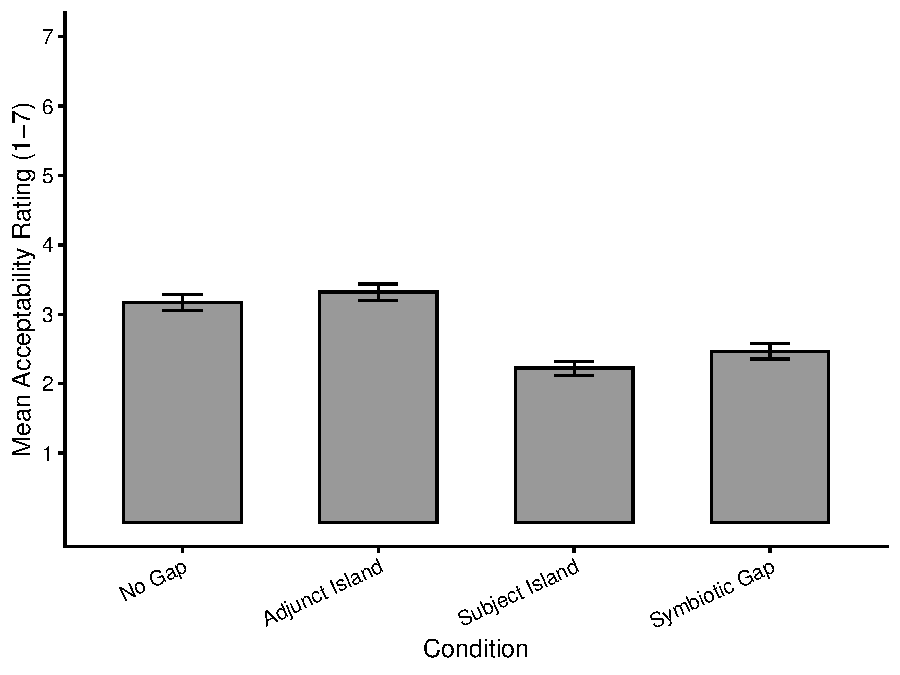
\includegraphics[width=0.75\textwidth]{../../Figures/symbiotic-gaps/experiment-1/Symbiotic Gaps 2x2 - Mean Acceptability by Condition.pdf}
\caption{Mean acceptability ratings (1--7) by condition. Error bars indicate standard errors.}
\label{fig:means}
\end{figure}

\begin{figure}[ht]
\centering
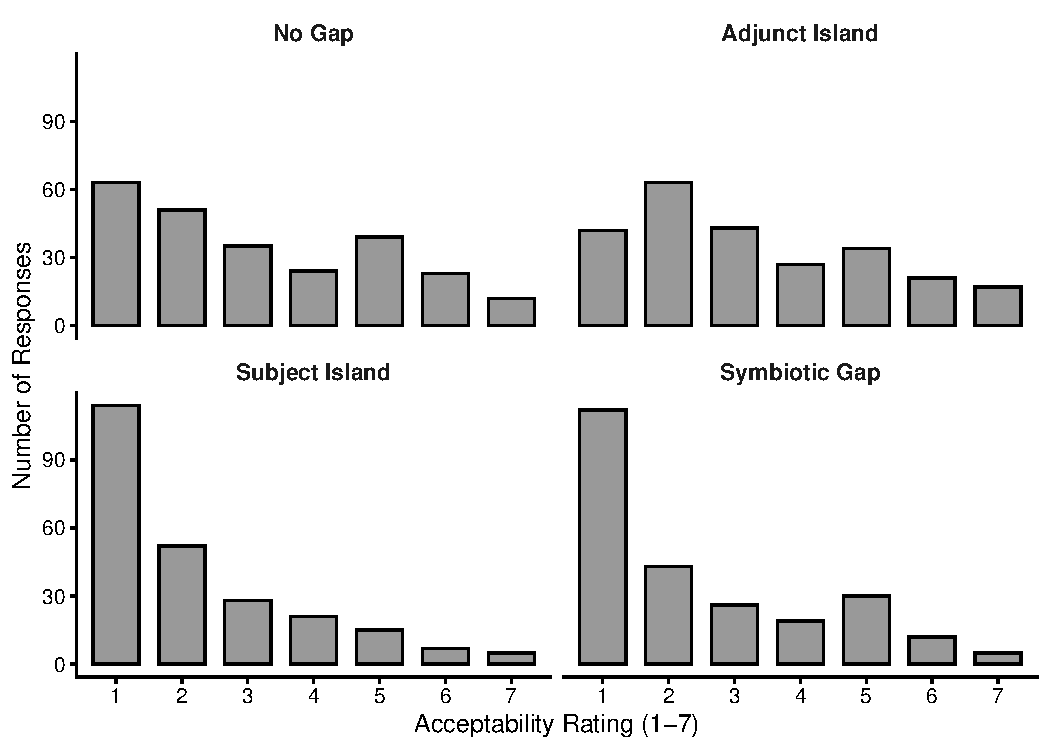
\includegraphics[width=0.85\textwidth]{../../Figures/symbiotic-gaps/experiment-1/Symbiotic Gaps 2x2 - Rating Distributions by Condition.pdf}
\caption{Distribution of acceptability ratings by condition. The Subject Island and Symbiotic Gap conditions show heavy concentration at the low end of the scale.}
\label{fig:distributions}
\end{figure}

A cumulative link mixed model (CLMM) was fit to the ordinal ratings with subject gap, adjunct gap, and their interaction as fixed effects (sum-coded, $\pm 0.5$), and random intercepts for participants ($N = 43$) and items ($N = 24$). The full results are reported in Table~\ref{tab:clmm}.

\begin{table}[ht]
\centering
\caption{Cumulative link mixed model results for Experiment 1.}
\label{tab:clmm}
\begin{tabular}{l r r r r}
\toprule
\textbf{Fixed effects} & \textbf{Estimate} & \textbf{SE} & $\boldsymbol{z}$ & $\boldsymbol{p}$ \\
\midrule
Subject gap & $-1.38$ & 0.13 & $-10.54$ & $< .001$ \\
Adjunct gap & $0.33$ & 0.12 & $2.64$ & $.008$ \\
Subject gap $\times$ Adjunct gap & $0.04$ & 0.25 & $0.15$ & $.882$ \\
\midrule
\textbf{Random effects} & \multicolumn{2}{c}{\textbf{Variance}} & & \\
\midrule
Participant & \multicolumn{2}{c}{1.99} & & \\
Item & \multicolumn{2}{c}{0.35} & & \\
\midrule
\textbf{Pairwise comparisons (Tukey)} & \textbf{Estimate} & \textbf{SE} & $\boldsymbol{z}$ & $\boldsymbol{p}$ \\
\midrule
No Gap -- Adjunct Island & $-0.31$ & 0.17 & $-1.83$ & $.261$ \\
No Gap -- Subject Island & $1.40$ & 0.18 & $7.64$ & $< .001$ \\
No Gap -- Symbiotic Gap & $1.05$ & 0.18 & $5.95$ & $< .001$ \\
Adjunct Island -- Subject Island & $1.71$ & 0.18 & $9.32$ & $< .001$ \\
Adjunct Island -- Symbiotic Gap & $1.36$ & 0.18 & $7.62$ & $< .001$ \\
Subject Island -- Symbiotic Gap & $-0.34$ & 0.18 & $-1.89$ & $.234$ \\
\bottomrule
\end{tabular}
\end{table}

The presence of a gap in the subject position significantly reduced acceptability ($b = -1.38$, $z = -10.54$, $p < .001$). The presence of a gap in the adjunct position had a small but significant positive effect ($b = 0.33$, $z = 2.64$, $p = .008$). Crucially, the interaction between the two factors was negligible and not significant ($b = 0.04$, $z = 0.15$, $p = .882$), indicating that the combined effect of the two gaps on acceptability was purely additive.

Tukey-adjusted pairwise comparisons confirmed that the four conditions fall into two groups. The No Gap and Adjunct Island conditions did not differ from each other ($z = -1.83$, $p = .261$), nor did the Subject Island and Symbiotic Gap conditions ($z = -1.89$, $p = .234$). All comparisons across these two groups were highly significant (all $p < .001$).

\FloatBarrier
\subsection{Discussion}\label{sec:exp-discussion}

The results of Experiment 1 provide no evidence for the amelioration effect that the symbiotic gap hypothesis predicts. If combining a subject gap and an adjunct gap produced a mutual licensing relationship between the two gap sites, as \citeauthor{levine2003} propose, this should have been reflected in a superadditive interaction: the Symbiotic Gap condition should have received higher ratings than the additive combination of the individual gap penalties would predict. Instead, the interaction term was near zero ($b = 0.04$, $p = .882$). The Symbiotic Gap condition ($M = 2.47$) was rated only marginally above the Subject Island condition ($M = 2.22$), and this small difference is fully accounted for by the additive contribution of the adjunct gap. Adding an adjunct gap to a sentence with a subject island violation does not yield any special improvement; it provides the same small boost that an adjunct gap provides in the absence of a subject island violation.

The pattern that emerges is one of simple additivity: subject gaps impose a substantial penalty, adjunct gaps provide a modest boost, and the combination of the two in a symbiotic gap configuration shows no amelioration beyond what these independent effects predict. The fact that the Symbiotic Gap condition patterned with the Subject Island condition indicates that participants treated symbiotic gap sentences as island violations rather than as well-formed multiple-gap constructions.

One question that Experiment 1 leaves open concerns the role of the matrix gap. As noted in Section~\ref{sec:background}, parasitic gap constructions typically involve a gap in the matrix verb's complement position, which licenses the parasitic gap. If the low acceptability of symbiotic gaps reflects the absence of such a licensing gap, then introducing a matrix gap should improve acceptability. Experiment 2 tests this prediction by extending the design to include a matrix gap factor.

%% ==========================================================
%% SECTION 4: EXPERIMENT 2
%% ==========================================================

\section{Experiment 2}\label{sec:experiment2}

Experiment 1 established that symbiotic gap sentences are rated as poorly as subject island violations. Experiment 2 extends this finding by adding a third factor, the presence or absence of a gap in the matrix verb's complement position. This allows us to test whether a matrix gap improves acceptability in sentences containing island-internal gaps, as movement-based analyses predict. The full $2 \times 2 \times 2$ design also allows us to examine the behavior of standard parasitic gap configurations alongside symbiotic gaps and three-gap sentences.

\subsection{Design}\label{sec:exp2-design}

The experiment crossed three binary factors: \textsc{subject gap} (present vs.\ absent), \textsc{matrix gap} (present vs.\ absent), and \textsc{adjunct gap} (present vs.\ absent). This yielded eight conditions, illustrated in (\ref{exp2-conditions}).

\pex\label{exp2-conditions}
\a\label{exp2-nogap} No Gap:\\
What kinds of games do programmers of \emph{computer software} dread testing \emph{the gameplay} before debugging \emph{the code}?
\a\label{exp2-matwh} Matrix Wh:\\
What kinds of games do programmers of \emph{computer software} dread testing \underline{\hspace{1em}} before debugging \emph{the code}?
\a\label{exp2-adjisl} Adjunct Island:\\
What kinds of games do programmers of \emph{computer software} dread testing \emph{the gameplay} before debugging \underline{\hspace{1em}}?
\a\label{exp2-adjpg} Adjunct PG:\\
What kinds of games do programmers of \emph{computer software} dread testing \underline{\hspace{1em}} before debugging \underline{\hspace{1em}}?
\a\label{exp2-subjisl} Subject Island:\\
What kinds of games do programmers of \underline{\hspace{1em}} dread testing \emph{the gameplay} before debugging \emph{the code}?
\a\label{exp2-subjpg} Subject PG:\\
What kinds of games do programmers of \underline{\hspace{1em}} dread testing \underline{\hspace{1em}} before debugging \emph{the code}?
\a\label{exp2-symgap} Symbiotic Gap:\\
What kinds of games do programmers of \underline{\hspace{1em}} dread testing \emph{the gameplay} before debugging \underline{\hspace{1em}}?
\a\label{exp2-threegap} Three Gaps:\\
What kinds of games do programmers of \underline{\hspace{1em}} dread testing \underline{\hspace{1em}} before debugging \underline{\hspace{1em}}?
\xe

\noindent The eight conditions can be organized into two halves. The first four conditions (\ref{exp2-nogap})--(\ref{exp2-adjpg}) lack a subject gap; these include the No Gap control, a standard matrix extraction, an adjunct island violation, and a standard adjunct parasitic gap configuration. The second four conditions (\ref{exp2-subjisl})--(\ref{exp2-threegap}) all contain a subject gap; these include a subject island violation, a subject parasitic gap configuration, the symbiotic gap configuration, and a three-gap sentence (with gaps in all three positions).

Movement-based analyses make two predictions for this design. First, the Symbiotic Gap condition should not be rated above either of the island conditions, since none of these sentences contains a gap in a position from which extraction can independently proceed. Second, adding a matrix gap should improve acceptability across both the adjunct gap and subject gap conditions, since the matrix gap provides a non-island position from which the \emph{wh}-phrase can be extracted, licensing parasitic gaps in either island. This prediction should be visible as a main effect of the matrix gap factor, and should be especially clear in the contrast between the Adjunct Island (\ref{exp2-adjisl}) and Adjunct PG (\ref{exp2-adjpg}) conditions, and between the Subject Island (\ref{exp2-subjisl}) and Subject PG (\ref{exp2-subjpg}) conditions.

\subsection{Participants}\label{sec:exp2-participants}

Eighty native English speakers participated in the experiment.

\subsection{Materials and procedure}\label{sec:exp2-materials}

Twenty-four lexicalizations were constructed, each appearing in all eight conditions. The items were distributed across eight lists in a Latin Square design. Participants rated acceptability on a 1--7 scale as in Experiment 1.

\subsection{Data cleaning}\label{sec:exp2-cleaning}

The same exclusion criteria from Experiment 1 were applied. Individual trials with response times below 1500\,ms were removed, excluding 120 trials (6.3\% of the data). No participants were excluded for excessive trial loss or invariant responding. After cleaning, the dataset contained 80 participants, 24 items, and 1,800 trials (93.8\% of the original data).

\subsection{Results}\label{sec:exp2-results}

Mean acceptability ratings by condition are displayed in Figure~\ref{fig:exp2-means}. The eight conditions separate into three clusters. The Matrix Wh ($M = 4.91$) and Adjunct PG ($M = 4.86$) conditions were rated highest. The No Gap ($M = 2.68$) and Adjunct Island ($M = 2.90$) conditions occupied an intermediate range. The four subject gap conditions were all rated low: Subject Island ($M = 2.01$), Symbiotic Gap ($M = 2.02$), Subject PG ($M = 2.43$), and Three Gaps ($M = 2.48$). Figure~\ref{fig:exp2-distributions} shows the full distribution of ratings across conditions, and Figure~\ref{fig:exp2-interaction} displays the interaction between subject gap and adjunct gap at each level of the matrix gap factor.

\begin{figure}[ht]
\centering
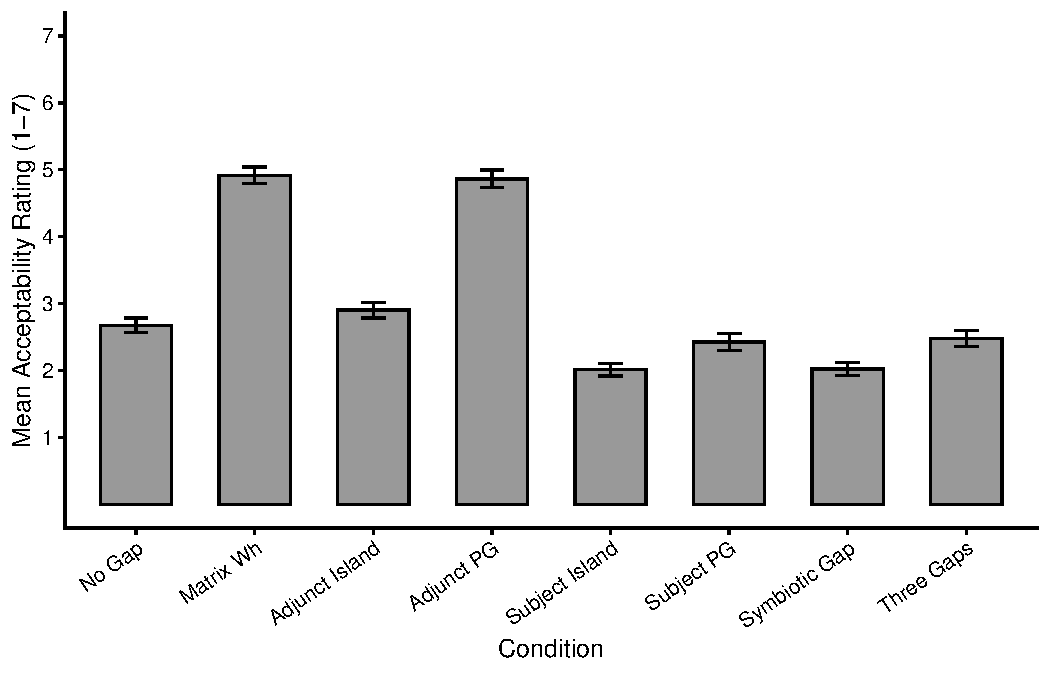
\includegraphics[width=0.85\textwidth]{../../Figures/symbiotic-gaps/experiment-2/Symbiotic Gaps 2x2x2 - Mean Acceptability by Condition.pdf}
\caption{Mean acceptability ratings (1--7) by condition in Experiment 2. Error bars indicate standard errors.}
\label{fig:exp2-means}
\end{figure}

\begin{figure}[ht]
\centering
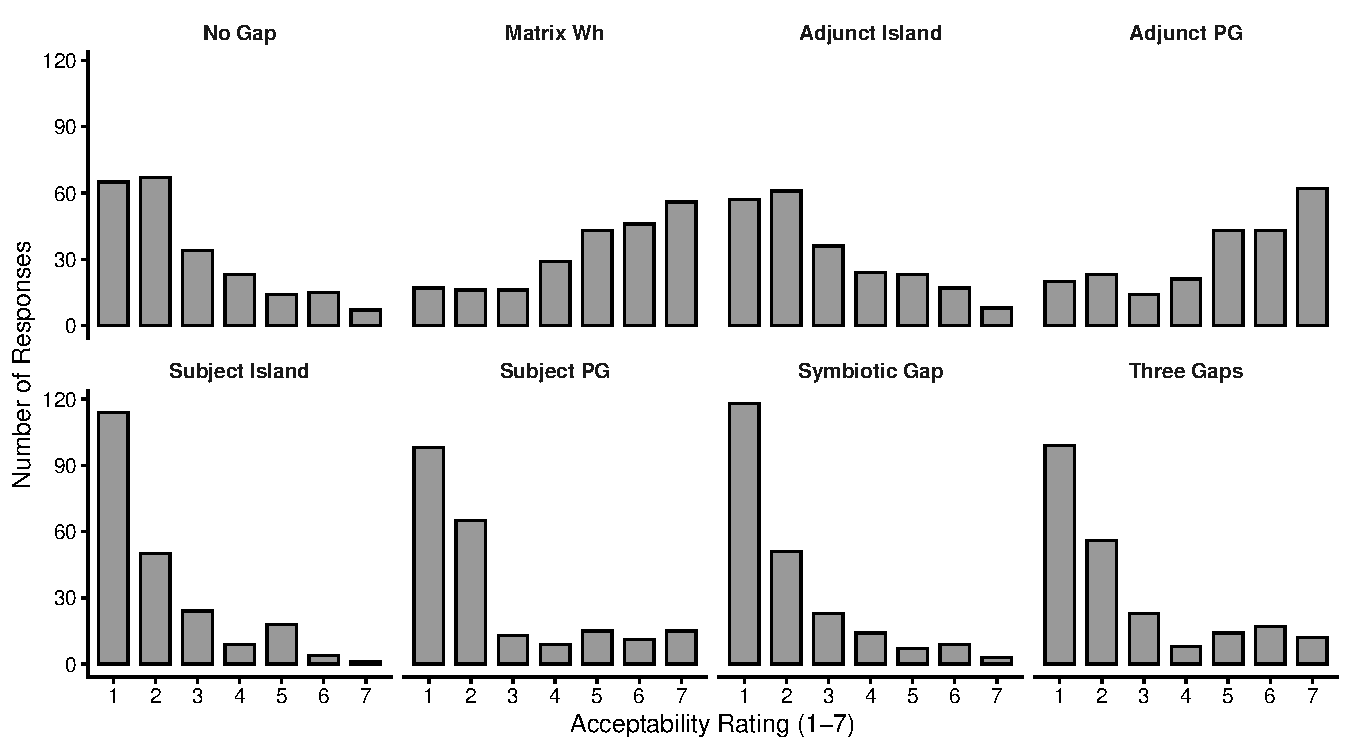
\includegraphics[width=0.95\textwidth]{../../Figures/symbiotic-gaps/experiment-2/Symbiotic Gaps 2x2x2 - Rating Distributions by Condition.pdf}
\caption{Distribution of acceptability ratings by condition in Experiment 2.}
\label{fig:exp2-distributions}
\end{figure}

\begin{figure}[ht]
\centering
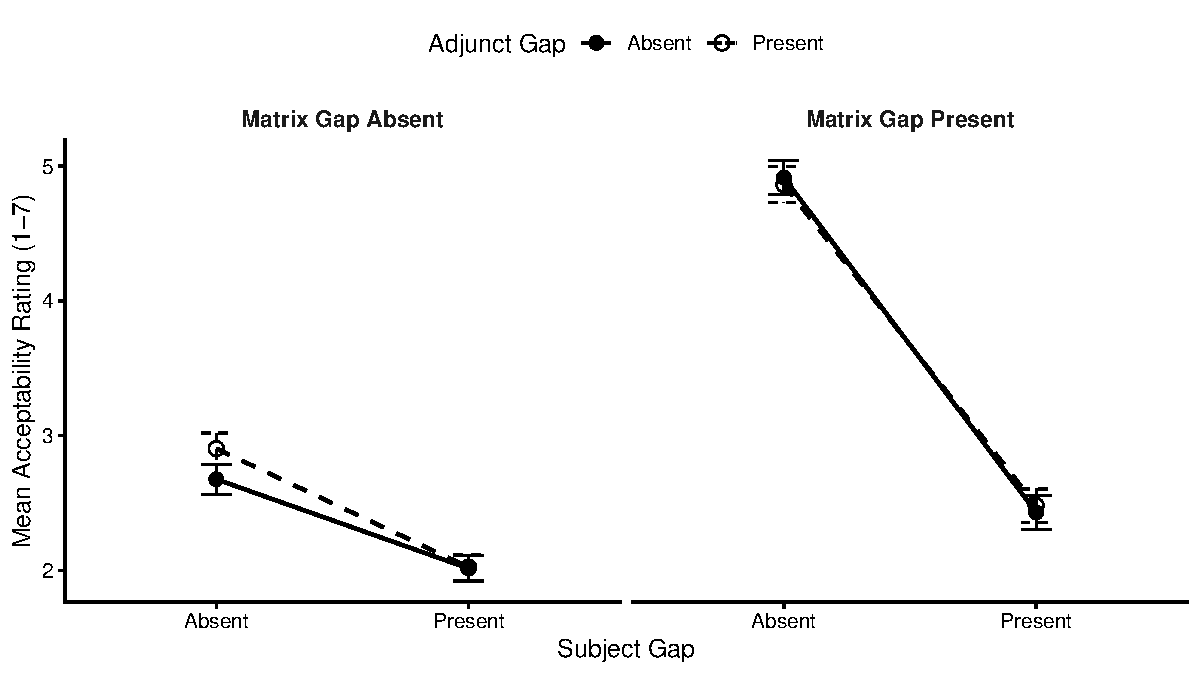
\includegraphics[width=0.95\textwidth]{../../Figures/symbiotic-gaps/experiment-2/Symbiotic Gaps 2x2x2 - Interaction Plot.pdf}
\caption{Interaction plot for Experiment 2. Mean acceptability as a function of subject gap and adjunct gap, faceted by matrix gap. The steep drop when a subject gap is introduced is attenuated by the matrix gap (right panel), but the adjunct gap (dashed vs.\ solid lines) has no effect in either panel.}
\label{fig:exp2-interaction}
\end{figure}

A cumulative link mixed model was fit to the ordinal ratings with subject gap, matrix gap, and adjunct gap as sum-coded fixed effects ($\pm 0.5$), all interactions, and random intercepts for participants ($N = 80$) and items ($N = 24$). The full results are reported in Table~\ref{tab:exp2-clmm}. Selected pairwise comparisons are reported in Table~\ref{tab:exp2-pairwise}.

\begin{table}[!ht]
\centering
\caption{Cumulative link mixed model results for Experiment 2.}
\label{tab:exp2-clmm}
\begin{tabular}{l r r r r}
\toprule
\textbf{Fixed effects} & \textbf{Estimate} & \textbf{SE} & $\boldsymbol{z}$ & $\boldsymbol{p}$ \\
\midrule
Subject gap & $-1.90$ & 0.10 & $-19.62$ & $< .001$ \\
Matrix gap & $1.31$ & 0.09 & $14.09$ & $< .001$ \\
Adjunct gap & $0.05$ & 0.09 & $0.53$ & $.599$ \\
Subject gap $\times$ Matrix gap & $-1.68$ & 0.18 & $-9.24$ & $< .001$ \\
Subject gap $\times$ Adjunct gap & $-0.08$ & 0.18 & $-0.46$ & $.646$ \\
Matrix gap $\times$ Adjunct gap & $-0.01$ & 0.18 & $-0.04$ & $.972$ \\
Subject $\times$ Matrix $\times$ Adjunct & $0.35$ & 0.35 & $1.00$ & $.317$ \\
\midrule
\textbf{Random effects} & \multicolumn{2}{c}{\textbf{Variance}} & & \\
\midrule
Participant & \multicolumn{2}{c}{1.04} & & \\
Item & \multicolumn{2}{c}{$< 0.001$} & & \\
\bottomrule
\end{tabular}
\end{table}

\begin{table}[!ht]
\centering
\caption{Selected pairwise comparisons for Experiment 2 (Tukey-adjusted).}
\label{tab:exp2-pairwise}
\begin{tabular}{l r r r r}
\toprule
\textbf{Contrast} & \textbf{Estimate} & \textbf{SE} & $\boldsymbol{z}$ & $\boldsymbol{p}$ \\
\midrule
\multicolumn{5}{l}{\emph{No subject gap}} \\
No Gap -- Adjunct Island & $-0.18$ & 0.17 & $-1.08$ & $.962$ \\
No Gap -- Matrix Wh & $-2.24$ & 0.18 & $-12.47$ & $< .001$ \\
Adjunct Island -- Adjunct PG & $-2.05$ & 0.18 & $-11.62$ & $< .001$ \\
Matrix Wh -- Adjunct PG & $0.004$ & 0.18 & $0.03$ & $1.000$ \\
\midrule
\multicolumn{5}{l}{\emph{Subject gap present}} \\
Subject Island -- Symbiotic Gap & $0.08$ & 0.18 & $0.43$ & $> .999$ \\
Subject Island -- Subject PG & $-0.38$ & 0.18 & $-2.08$ & $.427$ \\
Subject Island -- Three Gaps & $-0.47$ & 0.18 & $-2.59$ & $.158$ \\
Symbiotic Gap -- Three Gaps & $-0.55$ & 0.18 & $-3.04$ & $.049$ \\
Subject PG -- Three Gaps & $-0.09$ & 0.18 & $-0.51$ & $> .999$ \\
\bottomrule
\end{tabular}
\end{table}

Two main effects were significant. The presence of a subject gap substantially reduced acceptability ($b = -1.90$, $z = -19.62$, $p < .001$), and the presence of a matrix gap substantially increased it ($b = 1.31$, $z = 14.09$, $p < .001$). The adjunct gap had no significant main effect ($b = 0.05$, $z = 0.53$, $p = .599$).

The subject gap $\times$ matrix gap interaction was large and significant ($b = -1.68$, $z = -9.24$, $p < .001$). This interaction reflects the asymmetry visible in Figure~\ref{fig:exp2-interaction}: when no subject gap was present, the matrix gap produced a large boost in acceptability (No Gap $M = 2.68$ vs.\ Matrix Wh $M = 4.91$), but when a subject gap was present, the boost was sharply attenuated (Subject Island $M = 2.01$ vs.\ Subject PG $M = 2.43$). No other interaction reached significance: the subject gap $\times$ adjunct gap interaction ($p = .646$), the matrix gap $\times$ adjunct gap interaction ($p = .972$), and the three-way interaction ($p = .317$) were all negligible.

The pairwise comparisons in Table~\ref{tab:exp2-pairwise} reinforce these patterns. Among conditions without a subject gap, the No Gap and Adjunct Island conditions did not differ ($p = .962$), nor did the Matrix Wh and Adjunct PG conditions ($p = 1.000$), but the contrast between these two pairs was large: for instance, the Adjunct Island condition was rated far below the Adjunct PG condition ($z = -11.62$, $p < .001$), confirming that adding a matrix gap dramatically improves sentences with an adjunct gap. Among the four subject gap conditions, no pairwise comparison reached significance at the conventional level, with one exception: the Symbiotic Gap condition ($M = 2.02$) was rated significantly lower than the Three Gaps condition ($M = 2.48$; $z = -3.04$, $p = .049$). The Subject Island and Symbiotic Gap conditions were virtually identical ($M = 2.01$ vs.\ $M = 2.02$; $p > .999$).

\FloatBarrier
\subsection{Discussion}\label{sec:exp2-discussion}

Experiment 2 replicates and extends the central finding of Experiment 1. As in the first experiment, symbiotic gap sentences received low acceptability ratings that were indistinguishable from subject island violations ($p > .999$). The adjunct gap main effect, which was small but significant in Experiment 1, was not significant in Experiment 2 ($p = .599$), and the subject gap $\times$ adjunct gap interaction was again negligible ($p = .646$). There is no indication that the presence of an adjunct gap ameliorates a subject island violation in any way. This confirms the first prediction of the movement-based analyses: the Symbiotic Gap condition is no better than the island conditions.

The second prediction, that the matrix gap should improve acceptability across both adjunct gap and subject gap conditions, is strongly confirmed for the adjunct gap conditions. The Adjunct Island condition ($M = 2.90$), which contains an adjunct gap but no matrix gap, was rated far below the Adjunct PG condition ($M = 4.86$), which adds a matrix gap ($p < .001$). The Adjunct PG condition was rated as high as the simple matrix extraction condition (Matrix Wh, $M = 4.91$; $p = 1.000$), confirming that a properly licensed parasitic gap carries no additional processing cost. Adding a matrix gap to a sentence with an adjunct gap transforms it from an island violation into a fully acceptable parasitic gap construction.

For the subject gap conditions, the matrix gap's effect was in the predicted direction but sharply attenuated. The Subject PG condition ($M = 2.43$) was rated numerically above the Subject Island condition ($M = 2.01$), but this difference did not reach significance ($p = .427$). This attenuation is captured by the significant subject gap $\times$ matrix gap interaction ($b = -1.68$, $p < .001$) and is visible in the steep convergence of the lines in the right panel of Figure~\ref{fig:exp2-interaction}. The subject island violation appears to impose a penalty that largely overwhelms the benefit of a matrix gap.

The comparison between the Symbiotic Gap and Three Gaps conditions is particularly informative. These two conditions are identical except that the Three Gaps condition includes a matrix gap. The significant difference between them ($p = .049$) indicates that even in the context of a subject island violation, the matrix gap contributes some improvement in acceptability. The adjunct gap alone does not: the Symbiotic Gap condition ($M = 2.02$) was no better than the Subject Island condition ($M = 2.01$). This pattern is consistent with the view that parasitic gaps require a licensing gap in a non-island position, and that the adjunct gap in a symbiotic gap configuration, which lacks such a licensor, provides no benefit.

%% ==========================================================
%% SECTION 5: GENERAL DISCUSSION
%% ==========================================================

\section{General Discussion}\label{sec:discussion}

The two experiments reported here converge on a clear empirical conclusion: symbiotic gap sentences are not well-formed. In neither experiment did the presence of an adjunct gap produce any detectable amelioration of a subject island violation. The symbiotic gap configuration is judged as an island violation because that is what it is.

\subsection{The role of the matrix gap}\label{sec:matrix-gap-role}

Experiment 2 additionally revealed an asymmetry between the matrix gap and the adjunct gap. As discussed in Section~\ref{sec:exp2-discussion}, the matrix gap dramatically improved sentences with an adjunct gap but had a sharply attenuated effect in the presence of a subject gap. We take this attenuation to reflect the processing difficulty of these sentences. All subject gap conditions involve extraction from a complex subject, which independently degrades acceptability. Moreover, the Three Gaps condition requires the reader to track three gap-filler dependencies in a single sentence, a processing burden that likely masks the structural benefit of the matrix gap. The interpretation is supported by the consistent numerical trend in the predicted direction and by the significant contrast between the Symbiotic Gap and Three Gaps conditions ($p = .049$), which differ only in whether a matrix gap is present. This contrast demonstrates that the matrix gap plays a licensing role that the adjunct gap alone cannot fill.

\subsection{Implications for the theory of grammar}\label{sec:implications}

The findings reported here bear directly on the argument advanced by \citet{levine2003}. Recall that their case for HPSG rested on two claims: (i) that symbiotic gap sentences are well-formed, and (ii) that movement-based analyses cannot generate them while HPSG can. If both claims are correct, then the data favor HPSG. Our experiments undermine claim (i): speakers do not accept symbiotic gap sentences, rating them at the same level as unambiguous island violations.

With claim (i) removed, the theoretical implications reverse. The inability of movement-based analyses to generate symbiotic gap configurations is no longer a shortcoming; it is a correct prediction. The null operator/connectedness analysis (Section~\ref{sec:null-op}), the predicate modification approach (Section~\ref{sec:predication}), and sideward movement (Section~\ref{sec:sideward}) all predict that a gap in the matrix verb's complement position is required for the derivation to converge, and our results confirm this prediction.

Each of the three movement-based approaches can also accommodate the three-gap condition (\ref{exp2-threegap}), in which gaps appear in the subject, the matrix complement, and the adjunct. On the null operator/connectedness analysis, the \emph{wh}-phrase is extracted from the matrix complement position, forming a true chain that satisfies the connectedness condition. Null operators within the subject and adjunct each form their own chains, which connect to the true chain via the paths described by \citet{kayne1983}. On the predicate modification approach, the \emph{wh}-phrase undergoes successive-cyclic movement from the matrix complement position through Spec,$v$P to Spec,CP. The intermediate copy in Spec,$v$P provides the necessary element of type $\langle e,t \rangle$ for the adjunct's derived predicate to compose with via Predicate Modification; the subject-internal gap is licensed through a parallel mechanism: a null operator within the subject creates a derived predicate that composes with a copy of the \emph{wh}-phrase at the left periphery of $v$P, where the subject originates. On the sideward movement analysis, the NP is first merged into the adjunct and then copied sideward into the matrix complement position. From there, it is copied sideward again into the subject. The copy in the matrix complement position is then targeted a second time for $\bar{A}$-movement to Spec,CP. Because this copy occupies a non-island position, the movement is licit, and all three gaps are derived.

Conversely, the capacity of HPSG to generate symbiotic gap sentences becomes a liability. The Nonlocal Feature Principle, combined with the Subject Condition (Section~\ref{sec:hpsg}), predicts that (\ref{bg-symbiotic-a}) should be grammatical: the \textsc{slash} feature percolates from both the subject and adjunct gaps, the Subject Condition is satisfied because two elements on the verb's \textsc{arg-st} list are slashed, and the filler binds off the resulting \textsc{slash} value. Yet our participants consistently rejected sentences with this structure. The HPSG analysis, as formulated by \citeauthor{levine2003}, overgenerates.

This does not mean that HPSG is inherently incapable of capturing the relevant restriction. One could, for instance, revise the Subject Condition so that extraction from a subject requires a slashed \emph{complement} (rather than any slashed element on \textsc{arg-st}), which would block symbiotic gaps while still permitting standard parasitic gaps. Such a revision, however, would reintroduce an asymmetry between gap sites that is structurally parallel to the true-gap requirement of movement-based analyses. The theoretical advantage that \citeauthor{levine2003} claimed for HPSG, namely its ability to treat all gaps uniformly, would no longer hold.

%% ==========================================================
%% SECTION 6: CONCLUSION
%% ==========================================================

\section{Conclusion}\label{sec:conclusion}

This paper has presented two acceptability judgment experiments testing the empirical status of symbiotic gap constructions, the class of multiple-gap sentences that \citet{levine2003} advanced as evidence for HPSG over movement-based theories of grammar. Both experiments show that symbiotic gap sentences are rated no higher than subject island violations, and Experiment 2 additionally demonstrates that the matrix gap, not the adjunct gap, is the factor that licenses parasitic gaps in multiple-gap sentences. These results undermine the empirical foundation of \citeauthor{levine2003}'s argument: the inability of movement-based analyses to generate symbiotic gap configurations is a correct prediction, and the capacity of HPSG to generate them constitutes overgeneration. Parasitic gaps are genuinely parasitic: they depend on a gap in a non-island position for their licensing.

\printbibliography

\end{document}
